\section{RISE}

Like LIME, RISE\cite{Petsiuk2018rise} is a black box method and works by manipulating of the input images.

Instead of superpixels, RISE generates masks that are applied to the input images by multiplying the mask with the input image pixel values. Figure \ref{rise_mask0} and Figure \ref{rise_mask1} show two RISE masks applied to the same input image.

\begin{figure}[H]
    \centering
    \begin{subfigure}[t]{.32\textwidth}
        \centering
        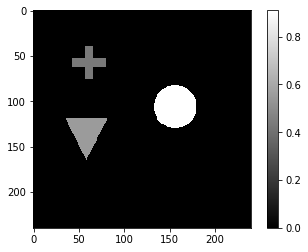
\includegraphics[width=\linewidth]{chapters/02_methods/images/rise/rise_original.png}
        \caption{Original image}
    \end{subfigure}\hfill%
    \begin{subfigure}[t]{.32\textwidth}
        \centering
        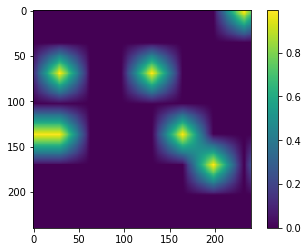
\includegraphics[width=\linewidth]{chapters/02_methods/images/rise/rise0_mask.png}
        \caption{RISE mask}
    \end{subfigure}\hfill%
    \begin{subfigure}[t]{.32\textwidth}
        \centering
        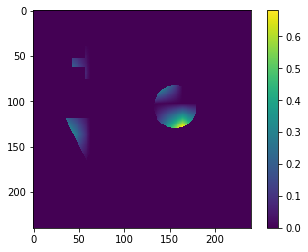
\includegraphics[width=\linewidth]{chapters/02_methods/images/rise/rise0_applied.png}
        \caption{RISE mask applied to original image by multiplication}
    \end{subfigure}
    \caption{By multiplication the input image (left) with a RISE mask (center), a modified input is generated (right).}
    \label{rise_mask0}
\end{figure}


\begin{figure}[H]
    \centering
    \begin{subfigure}[t]{.32\textwidth}
        \centering
        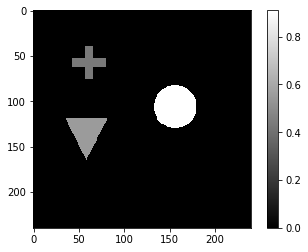
\includegraphics[width=\linewidth]{chapters/02_methods/images/rise/rise_original.png}
        \caption{Original image}
    \end{subfigure}\hfill%
    \begin{subfigure}[t]{.32\textwidth}
        \centering
        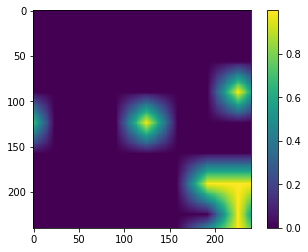
\includegraphics[width=\linewidth]{chapters/02_methods/images/rise/rise1_mask.png}
        \caption{RISE mask}
    \end{subfigure}\hfill%
    \begin{subfigure}[t]{.32\textwidth}
        \centering
        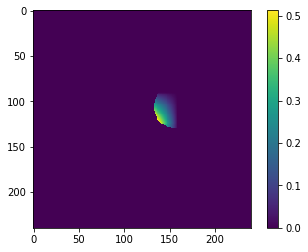
\includegraphics[width=\linewidth]{chapters/02_methods/images/rise/rise1_applied.png}
        \caption{RISE mask applied to original image by multiplication}
    \end{subfigure}
    \caption{By multiplication the input image (left) with a RISE mask (center), a modified input is generated (right). In comparison fo Figure \ref{rise_mask0}, this input image retains much less information.}
    \label{rise_mask1}
\end{figure}

The number of generated masks depend on the image resolution, e.g. for an image of size 240x240 pixels, 3000 masks generate good results. All masks are applied to the input image to generate new input images. The modified images are passed through the neural network and their classification scores for a specific class are recorded. A high classification score for a class on a modified input image means that the pixels preserved by the mask are important for the classification.

To visualize the results, the classification scores and masks are summed up and converted into a heat map. Figure \ref{rise_explanation} shows how the summing up works: The masks are multiplied with the classification score returned by running the masked image through the neural network. In Figure \ref{rise_explanation} for example, the leftmost mask was applied to an image, the image was run through the network and the network returned the value 0.7 for the first class. The next step is summing up all the values from the same cell into one matrix (image (c) in Figure \ref{rise_explanation}). In the actual implementation, the multiplication of the masks with the output values and summing up into one matrix is done with one matrix multiplication step.

\begin{figure}[H]
    \centering
    \begin{subfigure}[t]{\textwidth}
        \centering
        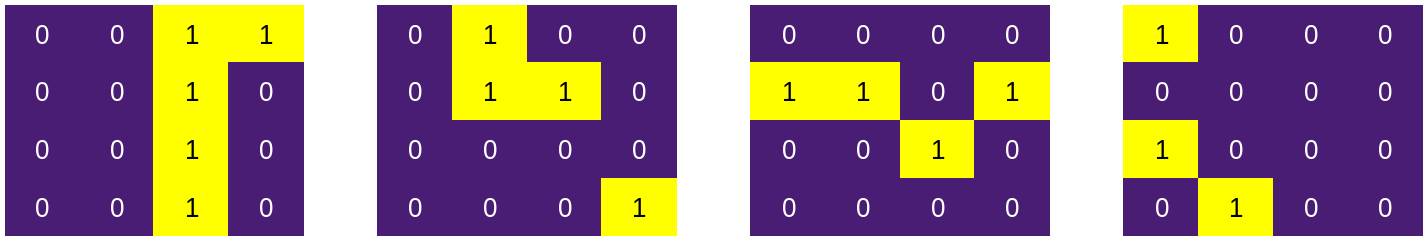
\includegraphics[width=\linewidth]{chapters/02_methods/images/rise/explain_rise_masks.png}
        \caption{Sample RISE masks}
    \end{subfigure}
    \begin{subfigure}[t]{\textwidth}
        \centering
        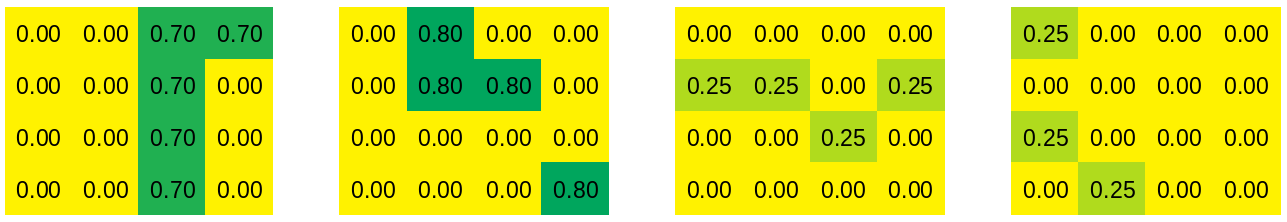
\includegraphics[width=\linewidth]{chapters/02_methods/images/rise/explain_rise_result.png}
        \caption{Masks multiplied by the classification value returned by the neural network after running the masked images through it}
    \end{subfigure}\hfill
    \begin{subfigure}[t]{.5\textwidth}
        \centering
        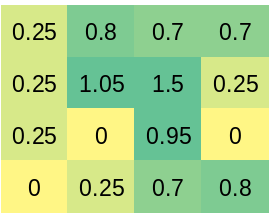
\includegraphics[width=\linewidth]{chapters/02_methods/images/rise/explain_rise_saliency.png}
        \caption{Saliency map generated by summing up all values for the same cell of the results in (b). E.g. second row second column is 0 + 0.8  + 0.25 + 0 = 1.05.}
    \end{subfigure}
    \caption{RISE masks (a) are multiplied by classification value returned by the network for the masked images (b). The same cell in theses matrices are summed up to generate a new matrix (c).}
    \label{rise_explanation}
\end{figure}

To visualize the generated matrix, the data is upscaled to the original image size and displayed as a heat map by mapping the values to a color map. Figure \ref{rise_example} shows some examples for visualization of the RISE output for specific classes.

\begin{figure}[H]
\centering
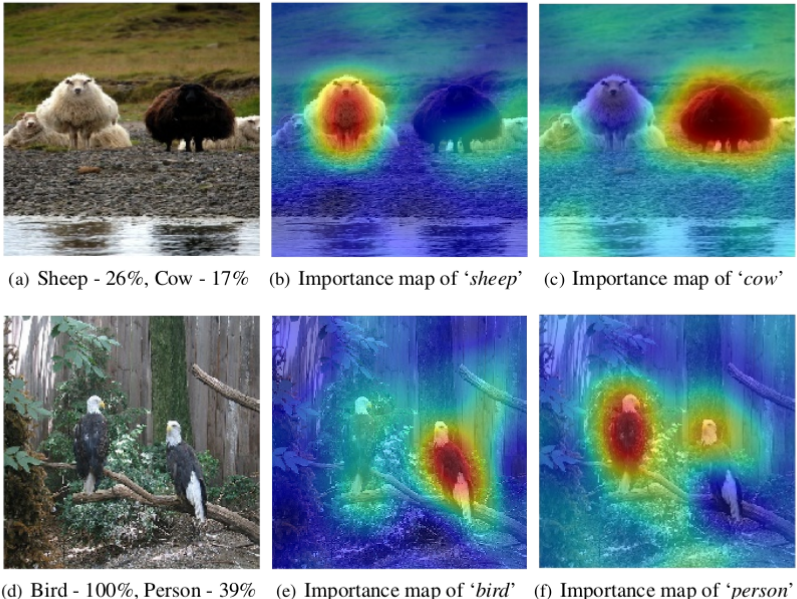
\includegraphics[width=12cm]{chapters/02_methods/images/rise/sheep.png}
\caption{Image from original paper explaining some classes}
\label{rise_example}
\end{figure}
